\hypertarget{ed2-introduction}{%
\chapter{Introduction}\label{ed2-introduction}}

Ce chapitre est consacré à la résolution numérique d'équations
différentielles \[
\dot{x} = f(t,x) \qquad , \qquad x(t_0)=x_0 \ .
\] La nécessité de développer des méthodes d'intégration numériques
vient du constat que seule une infime partie des équations
différentielles sont résolubles exactement. Or, on a parfois besoin de
connaître le plus précisément possible le comportement futur d'un
système dynamique~:

\begin{itemize}
\item
  soit en temps fini, par exemple pour déterminer la trajectoire d'une
  fusée pour la mise en orbite d'un satellite;
\item
  soit en temps \emph{long}, par exemple pour déterminer un cycle limite
  asymptotique (dynamique de population) ou bien se prononcer sur la
  stabilité de notre système solaire.
\end{itemize}

La méthode la plus connue est la \emph{méthode d'Euler} datant de 1768,
qui consiste à implémenter \[
x^{j+1} = x^j + {\Delta t}\, f(t_j,x^j) \qquad x^0 = x_0 
\] pour un pas de temps \({\Delta t}\) suffisamment petit. Cette méthode
appartient à la famille des méthodes \emph{explicites}, c'est-à-dire que
\(x^{j+1}\) est directement et explicitement défini en fonction de
\(x^{j}\). En 1824, Cauchy montre la convergence de cette méthode
lorsque le pas de temps \({\Delta t}\) tend vers 0, et prouve ainsi
l'existence et l'unicité des solutions (en fait, il utilise plutôt la
version \emph{implicite} de la méthode d'Euler).

Même si la méthode d'Euler suffit dans les cas simples, elle exige
parfois de recourir à des pas très faibles pour obtenir une précision
acceptable sur des temps longs (voir
\protect\hyperlink{ed2-sec_systRaides}{Systèmes raides (p.
\pageref*{ed2-sec_systRaides})}). Parfois, le compromis entre précision à
chaque itération et accumulation des erreurs d'arrondis devient même
impossible. De plus, cette méthode n'est pas adaptée à la simulation de
certains systèmes dont certaines propriétés cruciales (comme la
conservation de l'énergie) ne sont pas préservées (voir
\protect\hyperlink{ed2-sec_systHamiltoniens}{Systèmes Hamiltoniens (p.
\pageref*{ed2-sec_systHamiltoniens})}). Au cours des derniers siècles, les
scientifiques ont donc progressivement développé des méthodes de plus en
plus complexes et performantes~: schémas multi-pas d'ordre supérieur,
méthodes implicites, variation du pas, schémas symplectiques etc.

En fait, dans l'histoire des équations différentielles, c'est souvent la
mécanique céleste qui a été motrice des plus grandes avancées. Au milieu
du XIX\(^e\) siècle, les astronomes Adams et Le Verrier prédisent
mathématiquement l'existence et la position de la planète Neptune et
l'on entend parler pour la première fois de méthodes multi-pas. Ensuite,
les progrès se sont enchaînés au rythme des modèles physiques. La
première tendance a été de rechercher des schémas permettant toujours
plus de précision à pas plus grand. Parmi les dates clés, on peut citer
la publication en 1895 de la première méthode de Runge-Kutta par Runge,
puis en 1901, de la populaire méthode de Runge-Kutta d'ordre 4 par
Kutta, et ensuite en 1910, de l'\emph{extrapolation de Richardson}
permettant la montée en ordre et donc le recours à des pas plus grand
pour une même précision. Mais au milieu du XX\(^e\) siècle, on découvre
des systèmes, dits \emph{raides} (Hirschfelder, 1952), pour lesquels
cette montée en ordre ne suffit pas et pour lesquels il faut repenser de
nouveaux schémas (Dalquist, 1968). Enfin, à partir des années 80, les
scientifiques développent l'intégration numérique \emph{géométrique},
c'est-à-dire qui préservent les propriétés structurelles du système
(symétrie, conservation d'énergie etc.), utile en particulier pour la
simulation des systèmes hamiltoniens.

\hypertarget{ed2-objectifs-du-cours}{%
\chapter{Objectifs du cours}\label{ed2-objectifs-du-cours}}

Ce cours a pour but de sensibiliser aux problèmes apparaissant lors de
la simulation numérique des solutions d'équations différentielles, et de
donner les bases d'analyse d'erreur numérique. Pour un exposé plus
approfondi, on pourra par exemple se référer à (Demailly
\protect\hyperlink{ed2-ref-Dem06}{2006}).

En première lecture~:

\begin{itemize}
\item
  comprendre les limites d'un schéma d'Euler.
\item
  comprendre qu'un schéma numérique à un pas consiste à discrétiser une
  intégrale, en connaître quelques-uns autres que le schéma d'Euler.
\item
  comprendre les notions de consistance/convergence d'un schéma et leur
  ordre. Savoir montrer que le schéma d'Euler explicite est convergent
  d'ordre 1.
\end{itemize}

En deuxième lecture~:

\begin{itemize}
\item
  comprendre comment fonctionne un schéma implicite, comment
  l'implémenter, et quand il est pertinent de l'utiliser (syst\`emes raides ou non-lisses par exemple).
\item
savoir calculer l'ordre de consistance et montrer la convergence de
schémas de base.
\item
comprendre l'apport de schémas symplectiques pour les systèmes
hamiltoniens.
\item
  comprendre que la convergence est la combinaison de deux concepts~: la
  consistance et la stabilité\,; savoir utiliser ces notions pour
  évaluer l'impact des erreurs d'arrondi.
\end{itemize}

\hypertarget{ed2-limites-du-schuxe9ma-deuler}{%
\chapter{Limites du schéma d'Euler}\label{ed2-limites-du-schuxe9ma-deuler}}

La première limite du schéma d'Euler est qu'il est d'ordre 1,
c'est-à-dire qu'il produit une erreur en \({\Delta t}^2\) à chaque pas.
Nous verrons dans la suite des algorithmes d'ordre supérieur qui
permettent d'utiliser un pas plus grand pour une précision donnée. Mais
au delà de cette problématique, il existe des systèmes pour lesquels de
telles méthodes (même d'ordre supérieur) échouent. En voici deux
exemples célèbres.

\hypertarget{ed2-sec_systRaides}{%
\section{Systèmes raides}\label{ed2-sec_systRaides}}

La dénomination \emph{systèmes raides} a été introduite en 1952 par
Hirschfelder pour désigner des systèmes comprenant des dynamiques aux
constantes de temps très différentes. Dans ce cas, le pas nécessaire
pour simuler avec précision les dynamiques très rapides est si petit,
qu'il est alors impossible de simuler assez longtemps pour observer les
parties lentes. La particularité de ces systèmes est que cette
décroissance du pas apparaît alors que la solution est parfaitement
régulière, et non pas proche de singularités. C'est le cas des systèmes
linéaires \[
\dot{x} = A x + b
\] avec \(A\) de Hurwitz quand le rapport entre les parties réelles
maximales et minimales des valeurs propres devient très grand. Ce
phénomène peut notamment apparaître dans un simple système masse/ressort
\[
m\ddot{y} = -\rho \dot{y} - k y
\] qui se met sous la forme précédente avec
\(x=(y,\dot{y})\in \mathbb{R}^2\) et
\(A=\left(\begin{smallmatrix} 0&1\\-\dfrac{k}{m} & -\dfrac{\rho}{m} \end{smallmatrix}\right)\).
Lorsque les valeurs propres sont réelles (i.e.~\(\rho>2\sqrt{mk}\)),
leur rapport est donné par \[
\frac{1+\sqrt{1-4\dfrac{mk}{\rho^2}}}{1-\sqrt{1-4\dfrac{mk}{\rho^2}}}
\] qui explose lorsque \(\frac{mk}{\rho^2}\) tend vers 0. Par exemple,
lorsque les frottements sont très grands par rapport à la raideur du
ressort, ou bien lorsque \(\rho\) et \(k\) sont du même ordre de
grandeur et très grands.

Plus généralement, la coexistence de dynamiques très lentes à très
rapides apparaît en cinétique chimique ou en biologie. La réaction de
Robertson (1966) \begin{align*}
A & \stackrel{0.04}{\longrightarrow}  B \quad \text{(lente)} \\ 
B + B & \stackrel{3 \times 10^7}{\longrightarrow}  B + C \quad \text{(très rapide)}  \\
B + C & \stackrel{10^4}{\longrightarrow}  A + C  \quad \text{(rapide)} 
\end{align*} modélisée par \begin{align*}
\dot{x}_a &= -0.04 x_a + 10^4 x_bx_c \\
\dot{x}_b &= 0.04 x_a - 10^4 x_bx_c - 3\times 10^7 x_b^2\\
\dot{x}_c &= 3\times 10^7 x_b^2
\end{align*} en est un exemple classique, souvent utilisée pour tester
les schémas numériques. Il s'avère que pour ces systèmes, des schémas
dits \emph{implicites} performent beaucoup mieux car ils autorisent
l'utilisation de pas plus grands pour une même précision et plus de
stabilité (voir l'exercice
\protect\hyperlink{ed2-exo_exp_impl}{\emph{Explicite ou Implicite?} (p.
\pageref*{ed2-exo_exp_impl})}). Pour plus de détails voir (Hairer and Wanner
\protect\hyperlink{ed2-ref-Hairer96}{1996}). L'impossibilité de trouver un
pas approprié avec un schéma d'Euler explicite pour ce système, et la r\'esolution du probl\`eme par Euler implicite, sont aussi
illustrés dans le notebook Equations Differentielles II.ipynb. A  noter que l'utilisation des sch\'emas implicites est aussi cruciale dans la simulation des syt\`emes non-lisses ($f$ discontinue), qui apparaissent en m\'ecanique par exemple (frottement sec), voir l'exercice ci-dessus.

\hypertarget{ed2-sec_systHamiltoniens}{%
\section{Systèmes hamiltoniens}\label{ed2-sec_systHamiltoniens}}

La mécanique hamiltonienne permet typiquement de modéliser le
comportement de systèmes dont une certaine énergie est conservée au
cours du temps. Il peut s'agir par exemple de planètes en interaction
gravitationnelle, de particules en interaction électromagnétique, etc.

Par exemple, dans un problème à \(N\) corps en interaction
gravitationnelle, l'hamiltonien s'écrit\footnote{Pour obtenir
  l'hamiltonien, on commence par définir le lagrangien
  \(L(t,q,\dot{q})\), puis la quantité de mouvement
  \(p = \nabla_{\dot{q}} L(t,q,\dot{q})\), et enfin l'hamiltonien
  \(H(t,q,p)\) est obtenu par transformée de Legendre. Notons que dans
  ce cas général où \(H\) peut dépendre explicitement du temps (par
  exemple si de l'énergie est injectée ou prélevée par une action
  extérieure au système), on a
  \(\frac{d}{dt}H(t,q(t),p(t)) = \nabla_t H(t,q(t),p(t))\), donc
  l'hamiltonien varie selon cet effet extérieur, et n'est plus constant.}
\[
H(q,p) = \sum_{i=1}^{N} \frac{1}{2 m_i}p_i^\top p_i  - \sum_{1\leq i< k \leq N} G\frac{m_i m_j}{\|q_i-q_k\|}
\] où \(q_i\in \mathbb{R}^3\) désigne la position de chaque corps,
\(m_i\) sa masse, et \(p_i=m_i\dot{q}_i\in \mathbb{R}^3\) sa quantité de
mouvement. Le comportement de chaque corps est alors régi par la
dynamique hamiltonienne\footnote{L'application des lois de Newton
  donnerait directement \[
  m_i a_i = m_i \ddot{q_i} =  \sum_{k\neq i} F_k = -G \sum_{k\neq i} \frac{m_i m_j}{\|q_i-q_k\|^2}\frac{(q_i-q_k)}{\|q_i-q_k\|}
  \] où \(F_k\) sont les forces de gravitation exercées par chaque corps
  \(k\) sur le corps \(i\).} \begin{align*}
\dot{q}_i &= \nabla_{p_i} H(q,p) = \frac{1}{m_i} p_i \\
\dot{p}_i &= -\nabla_{q_i} H(q,p) = -G \sum_{k\neq i} \frac{m_i m_j}{\|q_i-q_k\|^3}(q_i-q_k)
\end{align*} On a alors le long des trajectoires \[
\frac{d}{dt}H(q(t),p(t)) = \left< \nabla_q H(t,q(t),p(t)), \dot{q} \right> + \left< \nabla_p H(t,q(t),p(t)), \dot{p} \right> = 0
\] et l'énergie \(H(q,p)\) est donc conservée.

Or, lorsqu'on essaye de simuler le système solaire avec un schéma
d'Euler (explicite), l'énergie augmente peu à peu à chaque révolution et
les trajectoires sont des spirales divergentes. Avec un schéma d'Euler
implicite, Jupiter et Saturne s'effondre vers le soleil en quelques ann\'ees (voir \protect\hyperlink{ed2-fig_systeme_solaire}{Figure~\ref*{ed2-fig_systeme_solaire} (p.
\pageref*{ed2-fig_systeme_solaire})}). Même des schémas d'ordre supérieur ne permettent
pas de simuler correctement ce système sur des temps ``courts'' sur
l'échelle de temps astronomique (à moins de prendre des pas
déraisonnablement petits). En fait, le problème c'est que ces méthodes
d'intégration ne préservent pas les propriétés structurelles des
solutions telles que la conservation de l'énergie. Il faut donc
développer des schémas particuliers, appelés \emph{symplectiques}, comme
illustré sur un simple oscillateur dans l'exercice
\protect\hyperlink{ed2-exo_symplectique}{\emph{Schéma symplectique} (p.
\pageref*{ed2-exo_symplectique})}. Pour aller plus loin sur ces méthodes,
voir (Hairer, Lubich, and Wanner
\protect\hyperlink{ed2-ref-Hairer10}{2010}). Un exemple simple de système à
deux corps est aussi donné dans le notebook Equations Differentielles
II.ipynb.

\begin{figure}
\hypertarget{ed2-fig_systeme_solaire}{%
\centering
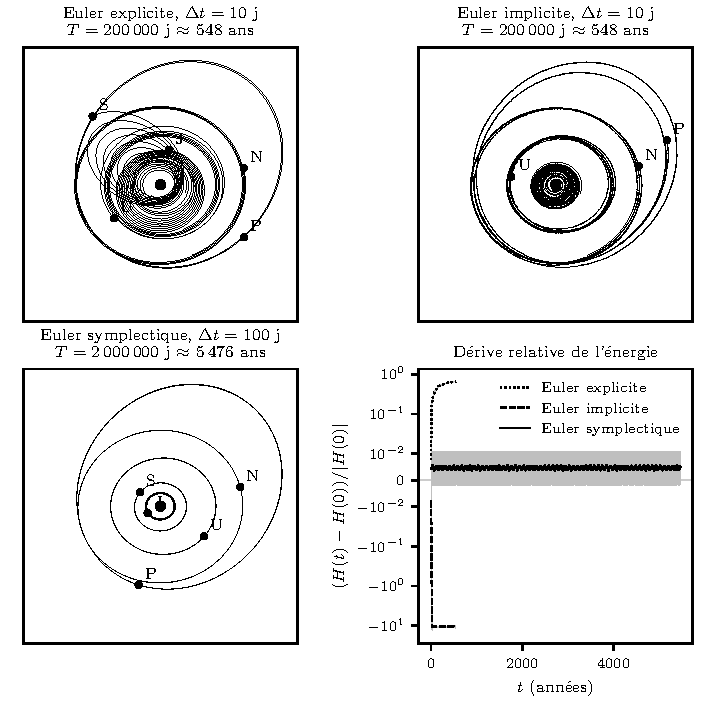
\includegraphics[width=\linewidth,height=0.55\textheight,keepaspectratio]{images/systeme_solaire.py.pdf}
\caption{Simulation du système solaire externe (Soleil, Jupiter, Saturne,
Uranus, Neptune, Pluton, données de (Hairer, Lubich, and Wanner
\protect\hyperlink{ed2-ref-Hairer10}{2010})) par les schémas d'Euler
explicite, implicite et symplectique, dans le référentiel du Soleil et
projetée dans le plan de l'écliptique. Avec Euler explicite, l'énergie augmente et les orbites de
Jupiter et Saturne s'ouvrent en spirale\,; avec Euler implicite, elle
diminue et les deux planètes tombent sur le Soleil en quelques
dizaines d'années. Le schéma symplectique, avec un pas dix fois plus
grand et un horizon dix fois plus long, conserve les orbites\,:
l'erreur sur l'énergie oscille à chaque révolution mais ne dérive pas.
En bas à droite, dérive relative de l'hamiltonien \(H\) (échelle
logarithmique de part et d'autre de \(\pm 10^{-2}\))\,: Euler explicite
gagne de l'énergie, Euler implicite en perd, massivement, jusqu'à la chute
de Jupiter\,; au-delà, le pas est bien trop grand pour résoudre l'orbite
numérique résiduelle et la simulation implicite n'a plus de sens.
%(en bas à droite, enveloppe de l'erreur relative sur l'hamiltonien\(H\)). 
%Le code générant cette figure est \texttt{images/systeme\_solaire.py}.
}\label{ed2-fig_systeme_solaire}
}
\end{figure}

\hypertarget{ed2-muxe9thodes-uxe0-un-pas}{%
\chapter{Méthodes à un pas}\label{ed2-muxe9thodes-uxe0-un-pas}}

\hypertarget{ed2-principe}{%
\section{Principe}\label{ed2-principe}}

Pour approximer les solutions d'une équation différentielle sur un
intervalle \([0,T]\), les méthodes numériques à un pas se basent sur la
représentation intégrale \[
x(t) = x_0 + \int_{t_0}^t f(s,x(s)) ds  = x_0 + \sum_{j=0}^{J-1} \int_{t_j}^{t_{j+1}}f(s,x(s)) ds
\] où \(t_0 < t_1 < \ldots < t_J\) avec \(t_J=T\). L'idée est
d'approximer les intégrales \(\int_{t_j}^{t_{j+1}}f(s,x(s))\) sur des
intervalles \([t_j,t_{j+1}]\) suffisamment petits.

Dans la suite, on note \(x^j\) l'approximation au temps \(t_j\) de la
valeur exacte \(x(t_j)\) et \({\Delta t}_j = t_{j+1}-t_j\) le \(j\)ème
pas de temps. L'idée est de calculer récursivement \[
x^{j+1} = x^j + {\Delta t}_j \Phi(t_j,x^j,{\Delta t}_j)
\] où \(\Phi(t_j,x^j,{\Delta t}_j)\) doit donc approximer \[
\frac{1}{t_{j+1}-t_j} \int_{t_j}^{t_{j+1}}f(s,x(s)) ds \ .
\] Les différentes méthodes de quadrature, i.e.~d'approximation de
l'intégrale, peuvent donc être mises à profit. La difficulté ici est que
seule la valeur initiale \(f(t_j,x(t_j))\) de \(f\) est connue (ou du
moins estimée) à l'itération \(j\), par \(f(t_j,x^j)\). On distingue
donc les méthodes \emph{explicites} où \(\Phi(t_j,x^j,{\Delta t}_j)\)
est écrite directement explicitement en fonction de la valeur initiale
\(x^j\), et les méthodes \emph{implicites} où cette expression n'est
connue qu'implicitement et des étapes intermédiaires de calcul sont
nécessaires.

\hypertarget{ed2-exemples}{%
\section{Exemples}\label{ed2-exemples}}

\begin{enumerate}
\def\labelenumi{\arabic{enumi}.}
\tightlist
\item
  Méthodes explicites:
\end{enumerate}

\begin{itemize}
\item
  Euler explicite: l'intégrale est approximée par l'aire d'un rectangle
  déterminé par la valeur initiale de \(f\) à \emph{gauche de
  l'intervalle}, i.e.\\
  \[
    x^{j+1} = x^j + {\Delta t}_j \, f(t_j,x^j) \ .
    \]
\item
  méthode de Heun~: l'intégrale est approximée par l'aire d'un trapèze
  déterminé par la valeur initiale de \(f\) et une approximation de sa
  valeur finale, i.e., \[
    x^{j+1} = x^j+\frac{{\Delta t}_j}{2}\Big(f(t_j,x^j) + f\big(t_{j+1},x^j+{\Delta t}_j f(t_j,x^j)\big) \Big) \ .
    \]
\item
  schéma de Runge--Kutta d'ordre 4: \[
  \left\{
  \begin{aligned}
  F_1 & = f(t_j,x^{j}) \\
  F_2 & = f\left(t_j+\frac{{\Delta t}_j}{2}, x^{j} + \frac{{\Delta t}_j}{2} F_1\right) \\
  F_3 & = f\left(t_j+\frac{{\Delta t}_j}{2}, x^{j} + \frac{{\Delta t}_j}{2} F_2\right) \\
  F_4 & = f(t_j + {\Delta t}_j, x^j + {\Delta t}_j F_3),
  \end{aligned}
  \right.
  \] et on pose \[
  x^{j+1} = x^{j} + {\Delta t}\, \frac{F_1 + 2F_2 + 2F_3 + F_4}{6} \ .
  \]
\end{itemize}

\begin{enumerate}
\def\labelenumi{\arabic{enumi}.}
\setcounter{enumi}{1}
\tightlist
\item
  Méthodes implicites:
\end{enumerate}

\begin{itemize}
\item
  Euler implicite~: l'intégrale est approximée par l'aire d'un rectangle
  déterminé par la valeur finale de \(f\) à \emph{droite de
  l'intervalle}, i.e.\\
  \[
    x^{j+1} = x^j + {\Delta t}_j \, f(t_{j+1},x^{j+1}) \ .
    \]
\item
  méthode des trapèzes (ou Crank--Nicolson)~: l'intégrale est approximée
  par l'aire du trapèze déterminé par les valeurs initiales et finales
  de \(f\), i.e.~ \[
  x^{j+1} = x^j+\frac{{\Delta t}_j}{2} \, \Big( f(t_j,x^j) + f(t_{j+1},x^{j+1})\Big) \ .
  \]
\item
  méthode du point milieu~: l'intégrale est approximée par l'aire d'un
  rectangle déterminé par une approximation de la valeur de \(f\) au
  milieu de l'intervale, i.e. \[
    x^{j+1} = x^j + {\Delta t}_j f\left(\frac{t_j+t_{j+1}}{2}, \frac{x^j+x^{j+1}}{2}\right) \ .
    \]
\end{itemize}

On peut bien sûr construire des méthodes plus compliquées et plus
précises pour des méthodes de Runge--Kutta d'ordre supérieur (explicites
ou implicites).

\hypertarget{ed2-sec_def_impl}{%
\section{\texorpdfstring{Définition implicite de
\(\Phi\)}{Définition implicite de \textbackslash Phi}}\label{ed2-sec_def_impl}}

Dans les schémas implicites, l'application \(\Phi\) est définie de
manière implicite. Par exemple, pour le schéma d'Euler, on a~: \[
\Phi(t_j,x^j,{\Delta t}_j) = f\Big(t_j + {\Delta t}_j, x^j + {\Delta t}_j\Phi(t_j,x^j,{\Delta t}_j) \Big).
\] Il faut donc s'assurer que \(\Phi\) est bien définie, c'est-à-dire
qu'il existe bien \(x^{j+1}\) tel que \[
x^{j+1} = x^j + {\Delta t}_j \, f(t_{j+1},x^{j+1}) \ .
\] Pour cela, nous pouvons voir \(x^{j+1}\) comme le point fixe de
l'application \(F_j\) définie par \[
F_j(x) = x^j + {\Delta t}_j \, f(t_{j+1},x) \ .
\] à \(x^j\), \({\Delta t}_j\), \(t_{j+1}\) fixés. L'existence (et
l'unicité) de ce point fixe peut alors être démontrée par le théorème de
point fixe de Banach. Si \(x\mapsto f(t_{j+1},x)\) est Lipschitzienne,
c'est-à-dire s'il existe \(L_j\) tel que \[
\|f(t_{j+1},x_a)-f(t_{j+1},x_b)\| \leq L_j \|x_a-x_b\| \qquad \forall (x_a,x_b)\in \mathbb{R}^n\times \mathbb{R}^n \ ,
\] alors \(F_j:\mathbb{R}^n \to \mathbb{R}^n\) est contractante pour un
pas de temps \({\Delta t}_j\) suffisamment petit puisque \[
\|F_j(x_a)-F_j(x_b)\| \leq  {\Delta t}_j L_j \|x_a-x_b\| \ .
\] Puisque \(\mathbb{R}^n\) est complet, on déduit par le théorème du
point fixe que \(x^{j+1}\) existe bien.

En pratique, on peut utiliser la méthode itérative de construction de ce
point fixe donnée par la preuve du théorème pour approcher \(x^{j+1}\).
Une stratégie est de partir de la valeur donnée par le schéma d'Euler
explicite \[
x^{j,0} = x^{j} + {\Delta t}_j f(t_j,x^{j})
\] et affiner ensuite par l'algorithme du point fixe en itérant \[
x^{j,k+1} = F(x^{j,k}) 
\] jusqu'à ce que l'évolution relative \[
\frac{x^{j,k+1}-x^{j,k}}{x^{j,0}}
\] devienne inférieure à un seuil choisi par l'utilisateur. Puisque la
suite \((x^{j,k})_{k\in \mathbb{N}}\) est de Cauchy, on sait que cette
algorithme s'arrête en un nombre fini d'itérations.

Notons que l'algorithme du point fixe n'est pas la seule façon de
résoudre l'équation \(x^{j+1} = F_j(x^{j+1})\)\,: c'est un système de
\(n\) équations non linéaires à \(n\) inconnues, \(G_j(x) = x - F_j(x) = 0\),
que l'on peut confier à n'importe quel solveur d'équations non linéaires,
typiquement la \emph{méthode de Newton} \[
x^{j,k+1} = x^{j,k} - \big(J_{G_j}(x^{j,k})\big)^{-1} G_j(x^{j,k}) \ ,
\] que l'on initialise là encore avec la prédiction du schéma explicite.
C'est ce que fait la fonction \texttt{scipy.optimize.fsolve} en Python,
et c'est la solution ``systématique''~: elle converge en quelques
itérations même lorsque \({\Delta t}_j L_j \geq 1\) et que \(F_j\) n'est
plus contractante, alors que l'algorithme du point fixe diverge. C'est
précisément dans ce régime, celui des pas de temps grands devant les
constantes de temps du système, que les schémas implicites sont
intéressants, et c'est pourquoi les solveurs implicites utilisent en
pratique une méthode de type Newton. Cette solution a ses limites~:

\begin{itemize}
\item
  chaque itération demande la jacobienne \(J_{G_j} = I - {\Delta t}_j J_f\)
  (calculée analytiquement, ou approchée par différences finies au prix de
  \(n\) évaluations supplémentaires de \(f\)) et la résolution d'un
  système linéaire de taille \(n\)\,: le coût par pas de temps croît vite
  avec la dimension\,;
\item
  Newton ne converge que depuis une initialisation suffisamment proche de
  la solution, et il n'y a aucune garantie si \({\Delta t}_j\) est
  trop grand~; le théorème de point fixe de Banach n'assure plus l'unicité
  de la solution, et le solveur peut converger vers une racine
  \emph{parasite} de \(G_j\), sans rien signaler. On l'observe
  par exemple sur le système raide de Robertson de la
  \protect\hyperlink{ed2-sec_systRaides}{section précédente (p.
  \pageref*{ed2-sec_systRaides})}, où un schéma d'Euler implicite résolu
  par \texttt{fsolve} converge pour \({\Delta t}=0{,}1\) vers une solution
  à concentrations négatives (voir le notebook Equations Differentielles II.ipynb)\,;
\item
  à l'inverse, si l'on choisit un pas de temps assez petit pour que
  \(F_j\) soit contractante, le point fixe est unique, l'algorithme de
  point fixe converge et n'exige aucune jacobienne~: c'est la méthode
  la plus simple, et elle suffit tant que l'on n'exploite pas la
  stabilité du schéma implicite pour prendre de grands pas.
\end{itemize}

Un tel schéma est plus lourd en terme de calculs qu'un algorithme
explicite mais il apporte en général plus de stabilité et permet souvent
d'utiliser un pas plus grand. C'est en particulier utile pour les
systèmes raides ou non-lisses, comme illustré dans l'exercice
\protect\hyperlink{ed2-exo_exp_impl}{\emph{Explicite ou Implicite?} (p.
\pageref*{ed2-exo_exp_impl})}.

\hypertarget{ed2-analyse-derreur}{%
\chapter{Analyse d'erreur}\label{ed2-analyse-derreur}}

L'objectif de l'analyse d'erreur \emph{a priori} est de donner une
estimation de l'erreur commise par la méthode numérique en fonction des
paramètres du problème (temps d'intégration, pas de temps, propriétés de
\(f\)). L'idée générale est de remarquer qu'à chaque pas de temps, on
commet une erreur d'intégration locale (erreur de troncature dans la
discrétisation de l'intégrale, à laquelle s'ajoutent souvent des erreurs
d'arrondi), et que ces erreurs locales s'accumulent au fil des pas. Le
contrôle de cette accumulation demande l'introduction d'une notion de
stabilité adéquate, alors que les erreurs locales sont liées à une
notion de consistance. L'alliance de stabilité et de consistante donne
une propriété de convergence qui est souhaitée lors de l'implémentation
de méthodes numériques.

\hypertarget{ed2-erreur-de-troncature-locale}{%
\section{Erreur de troncature
locale}\label{ed2-erreur-de-troncature-locale}}

L'erreur de troncature locale à l'itération \(j\) est l'erreur que l'on
commet en une seule itération lors de l'approximation de l'intégrale
pour passer de \(x^j\) à \(x^{j+1}\). C'est donc l'erreur théorique que
l'on obtiendrait si l'on appliquait le schéma numérique à la solution
exacte \(x(t_j)\). Elle est ainsi définie comme \[
\eta^{j+1} := \frac{x(t_{j+1}) - x(t_j) - {\Delta t}_j \Phi(t_j,x(t_j),{\Delta t}_j)}{{\Delta t}_j}.
\]

\hypertarget{ed2-def_consistance}{}
\addcontentsline{toc}{subsection}{Consistance}
\begin{definition}[Consistance]\label{ed2-def_consistance}
On note \({\Delta t}= \max_{0\le j\le J-1} {\Delta t}_j\) le pas de
temps maximal. On dit qu'une méthode numérique est \emph{consistante} si
\[
\lim_{{\Delta t}\to 0} \left( \max_{1\le j\le J} \|\eta^{j}\| \right) = 0 \ ,
\] et qu'elle est \emph{consistante d'ordre \(\geq p\)} s'il existe une
constante \(c_s\) telle que, pour tout \(0\le j\le J-1\), \[
\|\eta^{j+1}\| \le c_s \, ({\Delta t}_j)^{p} \ .
\] Une méthode est donc \emph{consistante d'ordre \(p\)} si elle est
consistante d'ordre \(\geq p\), mais pas \(\geq p+1\).
\end{definition}

\hypertarget{ed2-theo_CS_consistance}{}
\addcontentsline{toc}{subsection}{Condition nécessaire et suffisante de consistance}
\begin{theoreme}[Condition nécessaire et suffisante de consistance]\label{ed2-theo_CS_consistance}
Si \(\Phi\) est continue, alors le schéma est consistant si et seulement
si \[
\Phi(t,x,0) = f(t,x) \qquad \forall (t,x)\in \left[ 0,T \right]\times \mathbb{R}^n \ .
\]
\end{theoreme}

\hypertarget{ed2-duxe9monstration}{}
\begin{preuve}\label{ed2-duxe9monstration}
Soit \(C\) un ensemble fermé et borné tel que \(x(t)\in C\) pour tout
\(t\in \left[ 0,T \right]\). On note toujours
\({\Delta t}= \max_{0\le j\le J-1} {\Delta t}_j\). Par la représentation
intégrale des solutions, \[
x(t_{j+1}) = x(t_j) + \int_{t_j}^{t_{j+1}} f(x(s),s)ds
\] l'erreur de troncature locale s'écrit \[
\eta^{j+1} = \frac{1}{{\Delta t}_j}  \int_{t_j}^{t_{j+1}} \Big( f(s,x(s)) - \Phi(t_j,x(t_j),{\Delta t}_j) \Big)ds \ .
\] Si le schéma est consistant alors cette erreur tend vers 0 lorsque
\({\Delta t}\) tend vers 0 (pour n'importe quel système et n'importe
quelle trajectoire). Or, \[
\lim_{{\Delta t}\to 0} \frac{1}{{\Delta t}_j}  \int_{t_j}^{t_j+{\Delta t}} \Big( f(s,x(s)) - \Phi(t_j,x(t_j),{\Delta t}_j) \Big)ds = f(t_j,x(t_j)) - \Phi(t_j,x(t_j),0)
\] qui doit donc être nul.

Réciproquement, supposons \(\Phi(\cdot,\cdot,0)=f\). On doit montrer que
l'erreur de consistance tend vers 0 lorsque \({\Delta t}\) tend vers 0
(uniformément en \(j=1,\hdots,N\)). Soit \(\varepsilon >0\). Par la
continuité de \(\Phi\) et \(f\) et puisque \(\Phi(\cdot,\cdot,0)=f\), il
existe \(\Delta_1 >0\) tel que si \({\Delta t}\leq \Delta_1\), alors \[
\|\Phi(t,x,{\Delta t}_j) -f(t,x) \| \leq \varepsilon \qquad \forall (t,x) \in \left[ 0,T \right]\times C \quad \forall j=1,\hdots,N \ .
\] Donc \[
\|\eta^{j+1}\| \leq  \varepsilon + \frac{1}{{\Delta t}_j}  \int_{t_j}^{t_{j+1}} \big\| f(s,x(s)) - f(t_j,x(t_j)) \big\|ds \ .
\] Puisque \(s\mapsto f(s,x(s))\) est continue sur l'intervalle fermé et
borné \(\left[ 0,T \right]\), elle y est uniformément continue, donc il
existe \(\Delta_2 >0\) tel que si \({\Delta t}\leq \Delta_2\), \[
\big\| f(s,x(s)) - f(t_j,x(t_j)) \big\| \leq \varepsilon \qquad \forall s \in \left[ t_j,t_{j+1} \right]\quad \forall j=1,\hdots,N
\] et donc \(\|\eta^{j+1}\|\leq 2 \varepsilon\) pour tout \(j\). Le
schéma est donc bien consistant.\hfill$\blacksquare$
\end{preuve}

\hypertarget{ed2-ex_consistance}{}
\addcontentsline{toc}{subsubsection}{Schémas consistants}
\begin{exemple}[Schémas consistants]\label{ed2-ex_consistance}
Reprenons les exemples donnés plus haut.

\begin{itemize}
\item
  Euler explicite~: \(\Phi(t,x,{\Delta t})= f(t,x)\) indépendamment de
  \({\Delta t}\) donc la condition est trivialement satisfaite.
\item
  Méthode de Heun~:
  \(\Phi(t,x,{\Delta t}) = \frac{f(t,x) + f(t+{\Delta t},x+{\Delta t}f(t,x))}{2}\)
  donne bien \(f(t,x)\) si \({\Delta t}=0\).
\item
  Runge Kutta d'ordre 4~: lorsque \({\Delta t}=0\),
  \(F_1=F_2=F_3=F_4=f(t,x)\) donc
  \(\Phi(t,x,0) = \frac{F_1+2F_2+2F_3+F_4}{6}=f(t,x)\).
\end{itemize}

De même, la consistance des méthodes implicites s'obtiennent en
remarquant que \(x^{j+1}=x^{j}\) lorsque \({\Delta t}=0\).

Cette condition suffisante permet donc de prouver facilement le
caractère consistant d'un schéma. Cependant, en pratique, on s'intéresse
surtout à son ordre de consistance. Pour cela, l'erreur de consistance
se calcule souvent par des développements de Taylor des solutions
lorsque celles-ci sont suffisamment régulières, et la constante \(c_s\)
s'exprime alors comme une borne sur les dérivées des solutions. En fait,
on remarque que lorsque \(f\) est continue, la solution est \(C^1\) (par
définition de nos solutions). Mais puisque \(\dot{x}(t)=f(t,x(t))\),
\(\dot{x}\) hérite de la régularité de \(f\): si \(f\) est \(C^k\) alors
les solutions \(x\) sont \(C^{k+1}\). Le calcul de l'ordre de
consistance dans le cas dus schéma d'Euler explicite est donné
ci-dessous. Pour les autres schémas, voir l'exercice
\protect\hyperlink{ed2-exo_consist}{\emph{Consistance de schémas} (p.
\pageref*{ed2-exo_consist})}
\end{exemple}

\hypertarget{ed2-ex_consistance_Euler}{}
\addcontentsline{toc}{subsubsection}{Ordre de consistance du schéma d'Euler explicite}
\begin{exemple}[Ordre de consistance du schéma d'Euler explicite]\label{ed2-ex_consistance_Euler}
L'erreur de troncature s'écrit \[
\eta^{j+1} = \frac{x(t_j + {\Delta t}_j) - \Big( x(t_j) + {\Delta t}_j \, f(t_j,x(t_j)) \Big)}{{\Delta t}_j}.
\] Or, si \(f\) est \(C^1\), alors \(x\) est \(C^2\) et par application
la formule de Taylor avec reste intégral, on a \[
x(t_j + {\Delta t}_j) =  x(t_j) + {\Delta t}f(t_j,x(t_j))  + {\Delta t}_j^2 \int_{0}^{1} \ddot{x}(t_j+s{\Delta t}_j)  (1-s) ds ,
\] en utilisant \(\dot{x}(t_j)=f(t_j,x(t_j))\). Ceci donne donc \[
\|\eta^{j+1}\| \leq {\Delta t}_j  \int_{0}^{1} \ddot{x}(t_j+s{\Delta t}_j)  (1-s) ds \leq \frac{{\Delta t}_j}{2} \max_{t\in [t_j,t_{j+1}]} \|\ddot{x}(t)\| \leq \frac{{\Delta t}_j}{2} \max_{t\in [0,T]} \|\ddot{x}(t)\| \ .
\] Le schéma d'Euler explicite est donc consistant d'ordre \(\geq 1\)
avec \[
c_s= \frac{\max_{t\in [0,T]} \|\ddot{x}(t)\|}{2} \ .
\]

Notons qu'en utilisant \(\dot{x}(t) = f(t,x(t))\), \[
\ddot{x}(t) = \partial_t f(t,x(t)) + \partial_x f(t,x(t)) \cdot f(t,x(t)),
\] et on peut exprimer \(c_s\) en fonction de bornes sur \(x\) et sur
les dérivées de \(f\). Plus généralement, en dérivant successivement
lorsque \(f\) est \(C^k\), notons
\(f^{[k]} : \mathbb{R}\times \mathbb{R}^n \to \mathbb{R}^n\) la fonction
dépendant des dérivées successives de \(f\) telle que \[
x^{(k+1)}(t) = f^{[k]}(t,x(t)) \ .
\] On a alors le théorème suivant, généralisant les calculs précédents.
\end{exemple}

\hypertarget{ed2-theo_CS_consistance_ordre_p}{}
\addcontentsline{toc}{subsection}{\texorpdfstring{Condition nécessaire et suffisante de consistance d'ordre \(\geq p\)}{Condition nécessaire et suffisante de consistance d'ordre ≥ p}}
\begin{theoreme}[Condition nécessaire et suffisante de consistance d'ordre \(\geq p\)]\label{ed2-theo_CS_consistance_ordre_p}
Si \(\Phi\) et \(f\) sont \(C^p\) alors le schéma est consistant d'ordre
\(\geq p\) si et seulement si \[
\frac{\partial^k \Phi}{\partial {\Delta t}^k}(t,x,0) = \frac{1}{k+1}  f^{[k]}(t,x) \qquad \forall 0\leq k\leq p-1 \ , \quad \forall (t,x)\in \left[ 0,T \right]\times \mathbb{R}^n \ .
\]
\end{theoreme}

\hypertarget{ed2-duxe9monstration-1}{}
\begin{preuve}\label{ed2-duxe9monstration-1}
L'erreur de troncature s'écrit \[
\eta^{j+1} = \frac{x(t_j + {\Delta t}_j) - \Big( x(t_j) + {\Delta t}_j \, \Phi(t_j,x(t_j),{\Delta t}_j) \Big)}{{\Delta t}_j}.
\] Or, si \(f\) est \(C^p\), alors \(x\) est \(C^{p+1}\) et par
application la formule de Taylor avec reste intégral, on a
\begin{align*}
x(t_j + {\Delta t}_j) &= x(t_j) + \sum_{k=1}^p \frac{{\Delta t}_j^k}{k!}  x^{(k)} (t_j) +  \frac{{\Delta t}_j^{p+1}}{p!}\int_{0}^{1} x^{(p+1)}(t_j+s{\Delta t}_j)  (1-s)^p ds \\
&= x(t_j) + \sum_{k=0}^{p-1} \frac{{\Delta t}_j^{k+1}}{(k+1)!}  f^{[k]}(t_j,x(t_j)) +  \frac{{\Delta t}_j^{p+1}}{p!}\int_{0}^{1} x^{(p+1)}(t_j+s{\Delta t}_j)  (1-s)^p ds
\end{align*} Par ailleurs, puisque \(\Phi\) est \(C^p\), \[
\Phi(t,x,{\Delta t}) = \sum_{k=0}^{p-1} \frac{{\Delta t}^{k}}{k!}  \frac{\partial^k \Phi}{\partial {\Delta t}^k}(t,x,0) +  \frac{{\Delta t}^{p}}{(p-1)!}\int_{0}^{1} \frac{\partial^{p} \Phi}{\partial {\Delta t}^p}(t,x,t_j+s{\Delta t}_j)  (1-s)^{p-1} ds
\] Il s'ensuit que \[
\eta^{j+1} = \sum_{k=0}^{p-1} \frac{{\Delta t}_j^k}{k!} \left[ \frac{1}{k+1}  f^{[k]}(t_j,x(t_j)) - \frac{\partial^k \Phi}{\partial {\Delta t}^k}(t_j,x(t_j),0)\right] + {\Delta t}_j^p R_j
\] où \(R_j\) est borné (uniformément en \({\Delta t}_j\)) par
continuité de \(\frac{\partial^{p} \Phi}{\partial {\Delta t}^p}\) et
\(x^{(p+1)}\).

Maintenant, si le schéma est d'ordre \(\geq p\), alors
\(\frac{\eta^{j+1}}{{\Delta t}_j^p}\) doit rester borné lorsque
\({\Delta t}_j\) tend vers 0 et on obtient bien la condition du
théorème. Réciproquement, si la condition du théorème est vérifiée, on
obtient directement que \(\eta^{j+1}\) est borné en
\({\Delta t}_j^p\).\hfill$\blacksquare$
\end{preuve}

\hypertarget{ed2-ex_consistance_schemas}{}
\addcontentsline{toc}{subsubsection}{Ordre de consistance de schémas}
\begin{exemple}[Ordre de consistance de schémas]\label{ed2-ex_consistance_schemas}
On a vu que si \(f\) est \(C^1\), le schéma d'Euler explicite est
consistant d'ordre \(\geq 1\). On peut le retrouver ici en appliquant le
critère précédent pour \(p=1\) puisque \(\Phi(\cdot,\cdot,0)=f\).
Ensuite, si \(f\) est \(C^2\), on constate que \[
\frac{\partial\Phi}{\partial {\Delta t}}(t,x,0) = 0 \neq f^{[1]}(t,x) =\partial_t f(t,x) + \partial_x f(t,x) \cdot f(t,x)
\] donc le schéma d'Euler explicite est consistant d'ordre exactement
\(1\).

Par contre, toujours si \(f\) est \(C^2\), on constate que l'on a bien
pour le schéma de Heun \[
\frac{\partial\Phi}{\partial {\Delta t}}(t,x,0) =  f^{[1]}(t,x) =\partial_t f(t,x) + \partial_x f(t,x) \cdot f(t,x)
\] donc ce schéma est d'ordre \(\geq 2\). On peut vérifier que si \(f\)
est \(C^3\), le critère n'est pas vérifié à l'ordre supérieur donc il
est consistant d'ordre égal à 2.
\end{exemple}



\hypertarget{ed2-stabilituxe9}{%
\section{Stabilité}\label{ed2-stabilituxe9}}

Une fois que l'on a étudié l'erreur locale commise en une itération, on
s'intéresse à la manière dont elle va se propager au fur et à mesure des
itérations. Pour cela, la notion de stabilité quantifie la robustesse de
l'approximation numérique par rapport à l'accumulation des erreurs
locales et perturbations.

\hypertarget{ed2-def_stab}{}
\addcontentsline{toc}{subsection}{Stabilité}
\begin{definition}[Stabilité]\label{ed2-def_stab}
On dit qu'une méthode numérique est \emph{stable} s'il existe une
constante \(S(T) > 0\) (indépendente des \({\Delta t}_j\)) telle que,
pour toutes suites \(x = \{ x^j \}_{1 \leq j \leq J}\) et
\(z = \{ z^j \}_{1 \leq j \leq J}\) vérifiant \[
\left\{ \begin{aligned}
x^{j+1} & = x^j + {\Delta t}_j \Phi(t_j,x^j,{\Delta t}_j), \\
z^{j+1} & = z^j + {\Delta t}_j \Phi(t_j,z^j,{\Delta t}_j) + \delta^{j+1},
\end{aligned} \right.
\] on ait \[
\max_{1 \leq j \leq J} \| x^j - z^j\| \leq S(T) \, \Big( \|x^0 -z^0\| + \sum_{j = 1}^J  \|\delta^j\| \Big).
\]
\end{definition}

\hypertarget{ed2-theo_CS_stab}{}
\addcontentsline{toc}{subsection}{Condition suffisante de stabilité}
\begin{theoreme}[Condition suffisante de stabilité]\label{ed2-theo_CS_stab}
Si \(\Phi\) sont Lipschitziennes en \(x\), c'est-à-dire il existe
\(L>0\) tel que pour tout \(0\leq j\leq J\), \[
\|\Phi(t_j,x_a,{\Delta t}_j)-\Phi(t_j,x_b,{\Delta t}_j)\|\leq L \|x_a-x_b\| \qquad \forall (x_a,x_b)\in \mathbb{R}^n \times \mathbb{R}^n
\] alors le schéma est stable avec \(S(T)=e^{L T}\).
\end{theoreme}

\hypertarget{ed2-duxe9monstration-2}{}
\begin{preuve}\label{ed2-duxe9monstration-2}
On a alors \[
\| x^{j+1} - z^{j+1} \| \leq  \| \delta^{j+1} \| + (1 + {\Delta t}_j L) \| x^{j} - z^{j} \| \leq \| \delta^{j+1} \| +  e^{{\Delta t}_j L} \| x^{j} - z^{j} \| 
\] puisque \(1+x \leq e^{x}\) pour tout \(x\in \mathbb{R}\). Par
récurrence, on montre alors que pour tout \(1\leq j \leq J\), \[
\| x^{j} - z^{j} \| \leq e^{(t_j-t_0) L} \|x^0 -z^0\| + \sum_{k=1}^j e^{(t_j-t_k)L} \| \delta^{k} \|  \ .
\] Il s'ensuit que \[
\| x^{j} - z^{j} \| \leq e^{TL}\left(\|x^0 -z^0\|+ \sum_{k=1}^j \| \delta^{k} \|\right) \ ,
\] ce qui donne le résultat.\hfill$\blacksquare$
\end{preuve}

\hypertarget{ed2-convergence}{%
\section{Convergence}\label{ed2-convergence}}

La combinaison de consistance et de stabilité donne une propriété dite
de \emph{convergence} qui dit que l'erreur commise par le schéma par
rapport à la vraie solution converge vers 0 lorsque le pas de temps
converge vers 0. C'est une propriété cruciale pour un schéma numérique.

\hypertarget{ed2-def_conv}{}
\addcontentsline{toc}{subsection}{Convergence}
\begin{definition}[Convergence]\label{ed2-def_conv}
Soit \({\Delta t}= \max_{0 \leq j \leq J-1} {\Delta t}_j\). Un schéma
numérique est \emph{convergent} si \[
\lim_{{\Delta t}\to 0} \max_{1 \leq j \leq J} \|x^j - x(t_j)\| = 0
\] lorsque \(x^0 = x(t_0)\). S'il existe \(p\in \mathbb{N}_{>0}\) et
\(c_v>0\) (indépendent de \({\Delta t}\)) tel que \[
\max_{1 \leq j \leq J} \|x^j - x(t_j)\| \leq c_v ({\Delta t})^{p}
\] on dit que le schéma est \emph{convergent à l'ordre \(p\)}.
\end{definition}

\hypertarget{ed2-theo_Lax}{}
\addcontentsline{toc}{subsection}{Théorème de Lax}
\begin{theoreme}[Théorème de Lax]\label{ed2-theo_Lax}
Une méthode stable et consistante (à l'ordre \(p\)) est convergente (à
l'ordre \(p\)).
\end{theoreme}

\hypertarget{ed2-duxe9monstration-3}{}
\begin{preuve}\label{ed2-duxe9monstration-3}
Notons \(z^j=x(t_j)\). On remarque que \[
z^{j+1}  = z^j + {\Delta t}_j \Phi(t_j,z^j,{\Delta t}_j) + {\Delta t}_j\, \eta^{j+1},
\] où \(\eta\) est l'erreur de consistance. D'après la propriété de
stabilité, on a donc \[
\|x^j - x(t_j)\| \leq S(T) \,  \sum_{j = 1}^J {\Delta t}_{j-1}\, \|\eta^j\| \ ,
\] et par consistance \[
\|x^j - x(t_j)\| \leq S(T) \,  c_s \,  \sum_{j = 1}^J {\Delta t}_{j-1}\, ({\Delta t}_{j-1})^{p} \leq  c_s \, S(T) \, T \, ({\Delta t})^{p}  \ . 
\]\hfill$\blacksquare$
\end{preuve}

\hypertarget{ed2-theo_CS_conv}{}
\addcontentsline{toc}{subsection}{Condition suffisante de convergence}
\begin{theoreme}[Condition suffisante de convergence]\label{ed2-theo_CS_conv}
L'inconvénient du théorème de Lax est qu'il faut prouver la stabilité
pour obtenir la convergence. Or la seule condition suffisante dont nous
disposions à cet effet, est le caractère globalement Lipschitzien de
\(x\mapsto \Phi(t,x,{\Delta t})\). Mais il s'agit d'une condition très
forte. En fait, il est possible de prouver la convergence sous la
condition plus faible que \(x\mapsto \Phi(t,x,{\Delta t})\) est
``localement Lipschitzienne''~:

Si

\begin{enumerate}
\def\labelenumi{\arabic{enumi}.}
\item
  le schéma est consistant d'ordre \(p\),
\item
  pour tout boule fermée \(B\) de \(\mathbb{R}^n\), il existe \(L>0\),
  \({\Delta t}_m>0\) tels que pour tout \(t\in \left[ 0,T \right]\) et
  pour tout \({\Delta t}\in \left[ 0, {\Delta t}_m \right]\), \[
  \|\Phi(t_j,x_a,{\Delta t}_j)-\Phi(t_j,x_b,{\Delta t}_j)\|\leq L \|x_a-x_b\| \qquad \forall (x_a,x_b)\in B\times B 
  \]
\end{enumerate}

Alors il existe un pas de temps maximal \({\Delta t}_{\max}>0\) tel que
le schéma est convergent d'ordre \(p\).

L'hypothèse 2. est en particulier vérifiée si
\(x\mapsto \Phi(t,x,{\Delta t})\) est \(C^1\) d'après une version un peu
plus générale du théorème des accroissement finis.
\end{theoreme}

\hypertarget{ed2-ex_conv_Euler}{}
\addcontentsline{toc}{subsubsection}{Convergence du schéma d'Euler explicite}
\begin{exemple}[Convergence du schéma d'Euler explicite]\label{ed2-ex_conv_Euler}
On a déjà montré que le schéma d'Euler explicite est consistant d'ordre
1. Par ailleurs, si \(f\) est \(C^1\) par rapport à \(x\), alors
\(x\mapsto \Phi(t,x) = f(t,x,{\Delta t})\) est \(C^1\). Donc d'après le
théorème précédent, le schéma est convergent d'ordre 1.
\end{exemple}

Num\'eriquement, l'ordre de convergence des sch\'emas peut être visualis\'e en simulant une \'equation diff\'erentielle dont la solution analytique est connue, afin de tracer, en \'echelle log-log, l'erreur num\'erique de simulation en fonction du pas de temps\,: la pente de la courbe obtenue est l'ordre de convergence. C'est ce qui est fait sur la \protect\hyperlink{ed2-fig_ordre_schemas}{Figure~\ref*{ed2-fig_ordre_schemas} (p. \pageref*{ed2-fig_ordre_schemas})} pour les sch\'emas \`a un pas vus dans l'exercice \protect\hyperlink{ed2-exo_consist}{\emph{Consistance et ordre de sch\'emas} (p. \pageref*{ed2-exo_consist})}, sur le probl\`eme test \(\dot x = -x\), \(x(0)=1\), de solution \(x(t)=e^{-t}\). On retrouve les pentes \(1\), \(2\) et \(4\) d\'emontr\'ees analytiquement. Deux observations m\'eritent d'être soulign\'ees. D'une part, un sch\'ema implicite n'est pas plus pr\'ecis qu'un sch\'ema explicite\,: Euler implicite est d'ordre 1 comme Euler explicite, et ce que l'implicite apporte n'est pas de la pr\'ecision mais de la stabilit\'e (voir la \protect\hyperlink{ed2-sec_systRaides}{section sur les syst\`emes raides (p. \pageref*{ed2-sec_systRaides})}). D'autre part, pour le sch\'ema de Runge-Kutta 4, la courbe cesse de d\'ecro\^itre en dessous de \({\Delta t}\approx 10^{-3}\) et la pente ``casse''\,: l'erreur de troncature en \(({\Delta t})^4\) est alors devenue plus petite que la pr\'ecision de la machine, et ce sont les erreurs d'arrondi, accumul\'ees \`a chaque it\'eration, qui dominent. C'est l'objet de la section suivante.

\begin{figure}
\hypertarget{ed2-fig_ordre_schemas}{%
\centering
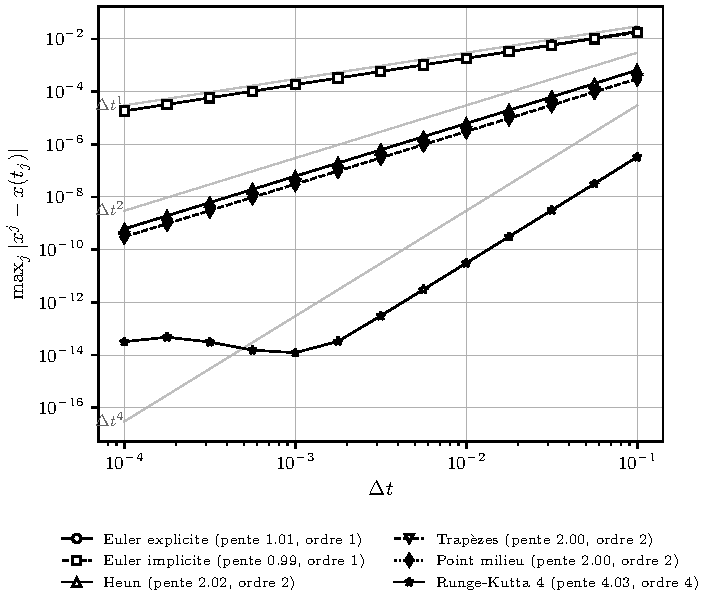
\includegraphics[width=\linewidth,height=0.5\textheight,keepaspectratio]{images/ordre_schemas.py.pdf}
\caption{Ordre de convergence exp\'erimental des sch\'emas \`a un pas du
cours sur le probl\`eme test \(\dot x = -x\), \(x(0)=1\), \(t\in[0,2]\)\,:
erreur globale \(\max_j |x^j-x(t_j)|\) en fonction du pas \({\Delta t}\)
(\'echelle log-log), et pente estim\'ee sur les six plus grands pas. Les
droites grises sont les r\'ef\'erences \(({\Delta t})^p\). 
%Le probl\`eme \'etant lin\'eaire, les sch\'emas des trap\`ezes et du point milieu co\"incident exactement. Pour Runge-Kutta 4, l'erreur sature autour de \(10^{-14}\) pour les petits pas\,: ce sont les erreurs d'arrondi. Le code g\'en\'erant cette figure est \texttt{images/ordre\_schemas.py}.
}\label{ed2-fig_ordre_schemas}
}
\end{figure}

\hypertarget{ed2-erreurs-darrondi-et-pas-optimal}{%
\section{Erreurs d'arrondi et pas
optimal}\label{ed2-erreurs-darrondi-et-pas-optimal}}

A chaque itération, lorsque la machine calcule \(x^{j+1}\), elle commet
en plus de l'erreur de troncature de l'intégrale des erreurs d'arrondi
de l'ordre de la précision machine. La solution obtenue est donc en fait
donnée par \[
\hat{x}^{j+1} = \hat{x}^j + {\Delta t}_j \left( \Phi(t_j,\hat{x}^j,{\Delta t}_j) + \rho^{j+1} \right)+ \varepsilon^{j+1}
\] au lieu de \[
x^{j+1} = x^j + {\Delta t}_j \Phi(t_j,x^j,{\Delta t}_j) \ ,
\] où \(\rho\) modélise l'erreur commise sur le calcul de \(\Phi\) et
\(\epsilon\) l'erreur sur l'addition finale. La stabilité nous donne
alors l'écart \[
\max_{0\leq j \leq J} \|x^j-\hat{x}^j\| \leq S(T) \sum_{j=1}^J {\Delta t}_{j-1} \|\rho^{j}\| + \|\varepsilon^{j}\| \ .
\] En considérant une borne \(\varepsilon\) des \(\varepsilon^{j}\) et
\(\rho\) des \(\rho^{j}\), on obtient \[
\max_{0\leq j \leq J} \|x^j-\hat{x}^j\| \leq S(T) (T\rho + J \varepsilon) \leq S(T) T \left(\rho + \frac{\varepsilon}{\min {\Delta t}_j} \right) \ ,
\] et donc finalement, en supposant l'algorithme convergent d'ordre
\(p\), \begin{align*}
\max_{0\leq j \leq J} \|x(t_j)-\hat{x}^j\| &\leq \max_{0\leq j \leq J} \|x(t_j)-x^j\| + \|x^j - \hat{x}^j\| \\
&\leq c_v (\max_j {\Delta t}_j)^p +  S(T) T \left(\rho + \frac{\varepsilon}{\min_j {\Delta t}_j} \right) \ .
\end{align*} Les paramètres \(\varepsilon\) et \(\rho\) sont typiquement
petits de l'ordre d'un facteur de la précision machine. Cependant, on
voit que plus le pas de temps décroit, plus il y a d'itérations et plus
les erreurs d'arrondi se propagent. D'un autre côté, plus il augmente,
plus les erreurs de quadrature augmentent. En supposant le pas constant,
il y a donc un pas ``optimal'\,' donné par \[
{\Delta t}_{opt} = \left( \frac{S(T) T\varepsilon}{c_vp}\right)^{\frac{1}{p+1}} \ .
\]

Ce ph\'enom\`ene est illustr\'e sur la \protect\hyperlink{ed2-fig_pas_optimal}{Figure~\ref*{ed2-fig_pas_optimal} (p. \pageref*{ed2-fig_pas_optimal})} avec le sch\'ema de Runge-Kutta 4 sur le probl\`eme test \(\dot x = -x\)\,: en diminuant le pas sur cinq ordres de grandeur, on voit l'erreur d\'ecro\^itre en \(({\Delta t})^4\), passer par un minimum autour de \(10^{-14}\), puis remonter. Plus l'ordre \(p\) est \'elev\'e, plus \({\Delta t}_{opt}\) est grand\,: un sch\'ema d'ordre \'elev\'e atteint la pr\'ecision machine avec un pas raisonnable, l\`a o\`u un sch\'ema d'ordre 1 demanderait un pas (et un nombre d'it\'erations) d\'eraisonnable. Il est donc illusoire de chercher \`a am\'eliorer la pr\'ecision en diminuant ind\'efiniment le pas\,: en pratique, on travaille toujours avec \({\Delta t}\gg {\Delta t}_{opt}\), et c'est le choix du sch\'ema et l'adaptation du pas (voir l'\protect\hyperlink{ed2-annexe-choix-du-pas-de-temps}{annexe (p. \pageref*{ed2-annexe-choix-du-pas-de-temps})}) qui permettent de contr\^oler l'erreur.

\begin{figure}
\hypertarget{ed2-fig_pas_optimal}{%
\centering
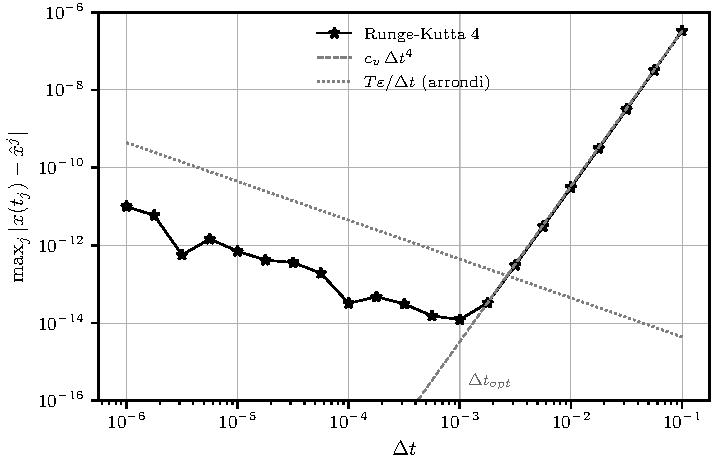
\includegraphics{images/pas_optimal.py.pdf}
\caption{Erreur globale du sch\'ema de Runge-Kutta 4 sur \(\dot x = -x\),
\(x(0)=1\), \(t\in[0,2]\) en fonction du pas, en double pr\'ecision
(\(\varepsilon\approx 2\cdot 10^{-16}\)). Pour les grands pas, l'erreur de
troncature \(c_v({\Delta t})^4\) domine\,; pour les petits pas, les erreurs
d'arrondi accumul\'ees sur les \(T/{\Delta t}\) it\'erations dominent et
l'erreur remonte lorsque le pas diminue. La borne \(T\varepsilon/{\Delta t}\)
du cours est un pire cas\,: en pratique les erreurs d'arrondi se compensent
partiellement et la remont\'ee observ\'ee est en dessous de cette borne. 
%Le pas optimal est au voisinage de la rencontre des deux asymptotes. Le code g\'en\'erant cette figure est \texttt{images/pas\_optimal.py}.
}\label{ed2-fig_pas_optimal}
}
\end{figure}

\hypertarget{ed2-annexe-choix-du-pas-de-temps}{%
\chapter{Annexe -- Choix du pas de
temps}\label{ed2-annexe-choix-du-pas-de-temps}}

Jusqu'à présent, on a présenté des schémas dépendant de pas de temps
\({\Delta t}_j\), sans jamais dire comment les choisir. Le plus simple
est de choisir un pas \({\Delta t}\) fixe mais il est difficile de
savoir à l'avance quel pas est nécessaire. En particulier, comment
savoir si la solution obtenue est suffisamment précise, sans connaître
la vraie\,?

\hypertarget{ed2-pas-fixe}{%
\section{Pas fixe}\label{ed2-pas-fixe}}

Une voie empirique est de fixer un pas, lancer la simulation, puis fixer
un pas plus petit, relancer la simulation, jusqu'à ce que les résultats
\emph{ne semble plus changer} (au sens de ce qui nous intéresse
d'observer). Notons que la connaissance des constantes de temps
présentes dans le système peut aider à fixer un premier ordre de
grandeur du pas. On pourrait aussi directement choisir le pas
\({\Delta t}_{opt}\) obtenu plus haut en prenant en compte les erreurs
d'arrondis. Mais les constantes \(c_v\) et \(S(T)\) sont souvent mal
connues et conservatives.

\hypertarget{ed2-adaptation-du-pas-de-temps}{%
\section{Adaptation du pas de
temps}\label{ed2-adaptation-du-pas-de-temps}}

Les méthodes à pas fixe exploitent la convergence des schémas, mais

\begin{itemize}
\item
  on ne peut pas prendre un pas de temps arbitrairement petit car on est
  contraint par le temps de simulation.
\item
  on n'a aucune idée de l'erreur commise et on n'est jamais sûr d'avoir
  la bonne solution.
\item
  l'utilisation d'un pas très petit peut n'être nécessaire qu'autour de
  certains points \emph{sensibles} (proches de singularités par exemple)
  et consomme des ressources inutiles ailleurs.
\end{itemize}

L'idée serait donc plutôt d'adapter la valeur du pas \({\Delta t}_j\) à
chaque itération. En d'autres termes, on se fixe une tolérance d'erreur
que l'on juge acceptable et on modifie le pas de temps en ligne, selon
si l'on estime être au-dessus ou en-dessous du seuil d'erreur. Mais cela
suppose d'avoir une idée de l'erreur commise\ldots{} Il existe justement
des moyens de l'estimer.

Tout d'abord, de quelle erreur parle-t-on\,?

\begin{itemize}
\item
  erreur \emph{globale}\,? L'idéal serait de contrôler
  \(\max_{0\leq j\leq N} \|x^j - x(t_j)\|\). Or la stabilité nous dit
  que \[
  \max_{0\leq j\leq N} \|x^j - x(t_j)\| \leq S(T) \,  \sum_{j = 1}^J {\Delta t}_{j-1}\, \|\eta^j\|
  \] avec \(\eta^j\) les erreurs de consistances locales. Donc si on se
  fixe une tolérance sur l'erreur globale \(\texttt{Tol}_g\), on a \[
  \|\eta^j\| \leq \frac{\texttt{Tol}_g}{TS(T)} \qquad \Longrightarrow \qquad \max_{0\leq j\leq N} \|x^j - x(t_j)\| \leq \texttt{Tol}_g \ .
  \] En d'autre termes, \(\texttt{Tol}_g\) nous fixe une erreur maximale
  \emph{locale} sur \(\eta^j\), à chaque itération. Notons cependant que
  cette borne ne prend pas en compte la propagation des erreurs
  d'arrondis~: plus \({\Delta t}\) diminue, plus l'erreur globale risque
  d'augmenter. Ce phénomène devrait donc en toute rigueur aussi nous
  donner un pas de temps minimal \({\Delta t}_{\min}\). Notons que tous
  ces calculs dépendent des constantes \(c_v\) et \(S(T)\) qui sont
  souvent mal connues ou très conservatives.
\item
  erreur (absolue) \emph{locale}\,? A chaque itération, une erreur
  locale est commise dûe à l'approximation de l'intégrale. Cette erreur
  est donnée par \[
  e^{j+1} = \tilde{x}(t_{j+1}) -x^{j+1} = \left(x^j + \int_{t_j}^{t_{j+1}} f(s,\tilde{x}(s))ds\right)
  \] où \(\tilde{x}\) est la solution de \(\dot{x}=f(t,x)\) qui serait
  initialisée à \(x^j\) au temps \(t_j\). Notons que si on avait
  \(x^j=x(t_j)\), on aurait exactement
  \(e^{j+1}={\Delta t}_j \eta^{j+1}\), où \(\eta^{j+1}\) est l'erreur de
  consistance. On se donne donc une tolérance d'erreur locale \[
  \|e^{j+1}\| \leq \texttt{Tol}_{abs} \ .
  \]
\item
  erreur \emph{relative}\,? Fixer une erreur absolue est parfois trop
  contraignant et n'a de sens que si les solutions gardent un certain
  ordre de grandeur. En effet, l'erreur acceptable quand la solution
  vaut 1000 n'est peut-être pas la même que lorsqu'elle vaut 1. On peut
  donc plutôt exiger une certaine erreur relative
  \(\texttt{Tol}_{rel}\), i.e., \[
  \frac{\|e^{j+1}\|}{\|x^j\|}\leq \texttt{Tol}_{rel} \ .
  \]
\end{itemize}

En général, les solvers assurent (approxivement) \[
\|e^{j+1}\| \leq \texttt{Tol}_{abs} + \texttt{Tol}_{rel} \|x^j\| \ .
\] Par défaut, dans les solvers de Numpy,
\(\texttt{Tol}_{abs} = 10^{-6}\) et \(\texttt{Tol}_{rel}= 10^{-3}\).

Mais pour cela nous devons trouver un moyen d'estimer l'erreur locale.
C'est souvent fait en utilisant une même méthode à deux pas différents
(par exemple \({\Delta t}_j\) et \({\Delta t}_j/2\)), ou bien en
imbriquant des schémas de Runge-Kutta d'ordres différents.

En fait, il est possible de montrer (exercice) que si \(f\) est \(C^1\),
on a pour un schéma d'Euler explicite \[
\|e^{j+1}\| = {\Delta t}_j \, \frac{\big\|f(t_{j+1},x^{j+1}) - f(t_j,x^j)\big\|}{2} + o({\Delta t}_j^2) \ 
\]

On peut donc estimer à chaque itération l'erreur commise \(e^{j+1}\) et
adapter le pas selon si celle-ci est inférieure ou supérieure au seuil
de tolérance. En effet, puisque l'on sait par ailleurs que
\(e^{j+1} = O({\Delta t}_j^2)\), une possible stratégie d'adaptation est
de prendre\\
\[
{\Delta t}_{new} = {\Delta t}_j \sqrt{\frac{\texttt{Tol}_{abs}}{\|e^{j+1}\|}}
\] (éventuellement avec une marge de sécurité)

La fonction correspondante
\begin{verbatim}
def solve_euler_explicit_variable_step(f, x0, t0, tf, dtmin, dtmax, atol):
  ...
  return t, x
\end{verbatim}
est fournie dans le notebook Equations Differentielles II.ipynb.
La \protect\hyperlink{ed2-fig_van_der_pol}{Figure~\ref*{ed2-fig_van_der_pol}
(p. \pageref*{ed2-fig_van_der_pol})} montre cette stratégie à l'\oe uvre
sur l'oscillateur de Van der Pol \[
\dot{y}_1 = y_2 \quad , \qquad \dot{y}_2 = \mu (1-y_1^2)\, y_2 - y_1
\] avec \(\mu = 10\) et \(y(0) = (2,0)\). Pour \(\mu\) grand, ce système
présente des \emph{oscillations de relaxation}\,: la solution alterne
entre des phases lentes, où elle suit de près une courbe en S dans le
plan de phase, et des sauts rapides quasi verticaux d'une branche de
cette courbe à l'autre. Le système est autonome\,: ce n'est pas le temps
qui rend \(f\) grande, c'est la trajectoire elle-même qui revient
périodiquement dans les régions de l'espace d'état (au voisinage de
\(y_1=\pm 1\)) où \(f\) et sa dérivée \(f^{[1]}\), donc l'erreur de
consistance, explosent. Le pas se resserre d'un facteur mille pendant
chaque saut puis se relâche jusqu'à \({\Delta t}_{\max}\) sur les
phases lentes, indéfiniment et en phase avec le cycle limite. Un pas
fixe devrait être choisi à la plus petite de ces valeurs partout. Notons
enfin que cette stratégie ne contrôle que l'erreur \emph{locale}\,: rien
ne garantit l'erreur globale, qui dépend de la constante de stabilité
\(S(T)\)\,; et que pour \(\mu\) plus grand encore, le système devient
franchement raide (voir la
\protect\hyperlink{ed2-sec_systRaides}{section sur les systèmes raides
(p. \pageref*{ed2-sec_systRaides})}) et le pas d'un schéma explicite
s'effondrerait pendant les sauts\,: il faudrait alors passer à un schéma
implicite.

\begin{figure}
\hypertarget{ed2-fig_van_der_pol}{%
\centering
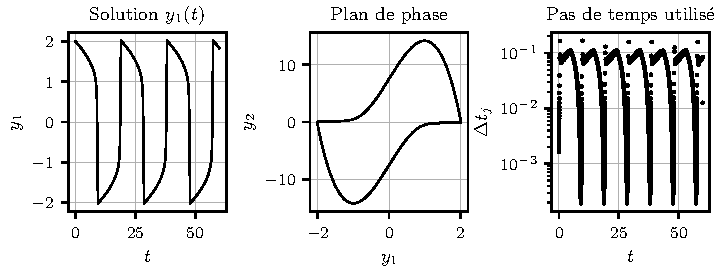
\includegraphics[width=\linewidth]{images/van_der_pol_pas_adaptatif.py.pdf}
\caption{Euler explicite à pas adaptatif sur l'oscillateur de Van der
Pol (\(\mu=10\), \(y(0)=(2,0)\), \(\texttt{Tol}_{abs}=10^{-4}\),
\({\Delta t}\in[10^{-6},0{,}2]\)). De gauche à droite\,: la solution
\(y_1(t)\), le plan de phase, et le pas \({\Delta t}_j\) retenu à chaque
itération (échelle logarithmique), qui se resserre à chaque saut du
cycle limite. 
%Le code générant cette figure est \texttt{images/van\_der\_pol\_pas\_adaptatif.py}.
}\label{ed2-fig_van_der_pol}
}
\end{figure}

\hypertarget{ed2-exercices}{%
\chapter{Exercices}\label{ed2-exercices}}

\hypertarget{ed2-exo_consist}{%
\section{Consistance et ordre de schémas}\label{ed2-exo_consist}}

Supposons \(f\) de classe \(C^2\). Montrer que~:

\hypertarget{ed2-consist-1}{%
\subsubsection*{Question 1}\label{ed2-consist-1}}

\addcontentsline{toc}{subsubsection}{Question 1}

le schéma de Heun est consistant d'ordre \(\geq 2\) et égal à 2 si \(f\)
est \(C^3\).\solref{ed2-answer-consist-1}

\hypertarget{ed2-consist-2}{%
\subsubsection*{Question 2}\label{ed2-consist-2}}

\addcontentsline{toc}{subsubsection}{Question 2}

le schéma d'Euler implicite est consistant d'ordre \(\geq 1\)\solref{ed2-answer-consist-2}

\hypertarget{ed2-consist-3}{%
\subsubsection*{Question 3}\label{ed2-consist-3}}

\addcontentsline{toc}{subsubsection}{Question 3}

la méthode des trapèzes est consistante d'ordre \(\geq 2\).\solref{ed2-answer-consist-3}

\hypertarget{ed2-consist-4}{%
\subsubsection*{Question 4}\label{ed2-consist-4}}

\addcontentsline{toc}{subsubsection}{Question 4}

le schéma du point milieu est consistant d'ordre \(\geq 2\).\solref{ed2-answer-consist-4}

\hypertarget{ed2-consist-5}{%
\subsubsection*{Question 5}\label{ed2-consist-5}}

\addcontentsline{toc}{subsubsection}{Question 5}

le schéma de Runge-Kutta d'ordre 4 est bien consistant d'ordre \(4\) si
\(f\) est \(C^5\).\solref{ed2-answer-consist-5}

On supposera le pas suffisamment petit pour que les schémas implicites
soient définis.

\hypertarget{ed2-conv}{%
\section{Convergence de schémas}\label{ed2-conv}}

Sous l'hypothèse que \(f\) est \(C^1\), montrer que les schémas de Heun
et d'Euler implicite sont convergents.\solref{ed2-answer-conv}

\hypertarget{ed2-exo_exp_impl}{%
\section{Explicite ou implicite\,?}\label{ed2-exo_exp_impl}}

Commençons par consid\'erer le cas des syst\`emes raides.

\hypertarget{ed2-impl-1}{%
\subsubsection*{Question 1}\label{ed2-impl-1}}

\addcontentsline{toc}{subsubsection}{Question 1}

Comparer les performances des schémas d'Euler implicites et explicites à
pas fixe dans le cas de \(\dot{x} = -\lambda x\), \(x(0)=1\), et
\(\dot{x} = \lambda x\), \(x(0)=1\), sur un horizon de temps \(T\)
donné.\solref{ed2-answer-impl-1}

\hypertarget{ed2-impl-2}{%
\subsubsection*{Question 2}\label{ed2-impl-2}}

\addcontentsline{toc}{subsubsection}{Question 2}

Lorsqu'on modélise des systèmes chimiques ou biologiques, on obtient
souvent des réactions aux constantes de temps très différentes. Vaut-il
mieux utiliser un schéma d'Euler implicite ou explicite pour simuler \[
\dot{x} = \left(
  \begin{matrix}
  -1 & 0 \\
  0 & -\mu
  \end{matrix}
  \right) x 
\] avec \(\mu >> 1\)\,?\solref{ed2-answer-impl-2}

\vspace{1em}
Consid\'erons maintenant le cas des syst\`emes non-lisses. Un solide freiné par un frottement sec (de Coulomb) subit une force de
module constant, toujours opposée à sa vitesse. En notant \(x\) la
vitesse, le modèle le plus simple est \[
\dot{x} = -\mathrm{sign}(x) \qquad , \qquad x(0) = x_0 \ ,
\] avec la convention \(\mathrm{sign}(0) = 0\). La fonction
\(\mathrm{sign}\) n'étant pas continue en 0, les théorèmes du chapitre
I ne s'appliquent pas tels quels\,: on cherche ici une solution
continue, dérivable sauf en un nombre fini d'instants, qui vérifie
l'équation partout ailleurs.

\hypertarget{ed2-impl-3}{%
\subsubsection*{Question 3}\label{ed2-impl-3}}

\addcontentsline{toc}{subsubsection}{Question 3 (Frottement sec)}

\begin{enumerate}
\def\labelenumi{\alph{enumi})}
\tightlist
\item
  Déterminer la solution pour \(x_0>0\), puis pour \(x_0\) quelconque.
  Qu'a-t-elle de remarquable par rapport à celle de
  \(\dot{x}=-\lambda x\)\,? Un tel comportement serait-il possible pour
  une équation \(\dot{x}=f(x)\) avec \(f\) continûment différentiable\,?
\item
  Ecrire le schéma d'Euler explicite de pas \({\Delta t}\) et décrire
  précisément le comportement de la suite \((x^j)\) à partir de
  \(x_0>0\), en particulier lorsqu'elle arrive au voisinage de 0.
  Diminuer le pas résout-il le problème\,?
\item
  Ecrire le schéma d'Euler implicite et montrer que, pour
  \(0<|x^j|\leq {\Delta t}\), l'équation définissant \(x^{j+1}\) n'a pas
  de solution avec la convention \(\mathrm{sign}(0)=0\). Montrer qu'en
  autorisant \(\mathrm{sign}(0)\) à prendre n'importe quelle valeur dans
  \([-1,1]\) (c'est la régularisation naturelle de la discontinuité),
  l'équation admet au contraire une unique solution pour tout \(x^j\),
  que l'on explicitera.
\item
  En déduire la suite \((x^j)\) produite par le schéma implicite et
  justifier qu'il résout le problème observé en b). 
  %Quelle propriété de
  %l'application \(x \mapsto x + {\Delta t}\,\mathrm{sign}(x)\), absente
  %de \(x \mapsto x - {\Delta t}\,\mathrm{sign}(x)\), est responsable de
  %cette différence\,?
\end{enumerate}\solref{ed2-answer-impl-3}

\hypertarget{ed2-exo_symplectique}{%
\section{Euler symplectique}\label{ed2-exo_symplectique}}

Pour \(\omega>0\) donné, considérons le système \[
\dot{x}_1 \;=\;  x_2
\quad ,\qquad 
\dot{x}_2(t)\;=\; -\omega^2 x_1
\] de condition initiale \(x(0)\;=\; (1,0)\). On rappelle que pour une
suite de la forme \(x^{j+1}=A x^j\) converge vers 0 si les valeurs
propres de \(A\) sont à l'intérieur du cercle unité et diverge si au
moins une valeur propre est à l'extérieur.

\hypertarget{ed2-symp-1}{%
\subsubsection*{Question 1}\label{ed2-symp-1}}

\addcontentsline{toc}{subsubsection}{Question 1}

Montrer que pour n'importe quel pas \({\Delta t}\) fixé, un schéma
d'Euler explicite donne une solution divergente, et un schéma d'Euler
implicite donne une solution qui converge vers 0. Lequel a raison\,?\solref{ed2-answer-symp-1}

On définit maintenant le schéma suivant qui ``mélange'\,' les schémas
d'Euler implicites et explicites~: \begin{align*}
x^{j+1}_1 &= x^{j}_1 + {\Delta t}\, x^{j}_2 \\
x^{j+1}_2 &= x^{j}_2 - {\Delta t}\, \omega^2 x^{j+1}_1
\end{align*}

\hypertarget{ed2-symp-2}{%
\subsubsection*{Question 2}\label{ed2-symp-2}}

\addcontentsline{toc}{subsubsection}{Question 2}

Montrer que la quantité
\(\omega^2 x_1^2 + x_2^2 +{\Delta t}\, \omega^2 x_1x_2\) est conservée.
Quelle est alors la forme des solutions obtenues dans le plan de phase
si \(\omega {\Delta t}<2\)\,? En déduire la pertinence de ce schéma. On
parle de schéma \emph{symplectique}, car il conserve les volumes.\solref{ed2-answer-symp-2}

\hypertarget{ed2-symp-3}{%
\subsubsection*{Question 3}\label{ed2-symp-3}}

\addcontentsline{toc}{subsubsection}{Question 3}

En écrivant le schéma sous la forme \(x^{j+1}=Ax^j\), montrer qu'il
diverge par contre si \({\Delta t}\, \omega > 2\).\solref{ed2-answer-symp-3}

\hypertarget{ed2-symp-4}{%
\subsubsection*{Question 4}\label{ed2-symp-4}}

\addcontentsline{toc}{subsubsection}{Question 4}

Plus généralement, proposer un schéma pour simuler un système
Hamiltonien du type \begin{align*}
\dot{q} &= \nabla_p H(q,p) \\
\dot{p} &= - \nabla_q H(q,p)
\end{align*} où \((q,p)\in \mathbb{R}^N \times \mathbb{R}^N\) sont les
positions généralisées et quantités de mouvement, \(H\) est le
Hamiltonien que l'on pourra vérifier être conservé le long des
trajectoires.\solref{ed2-answer-symp-4}

A noter que les conclusions de cet exercice sont les mêmes si l'on
utilise un schéma d'Euler implicite sur la première composante et un
schéma d'Euler explicite sur la deuxième. Ces deux schémas s'appellent
respectivement Euler symplectique A et B.

\hypertarget{ed2-ruxe9fuxe9rences}{%
\chapter{Références}\label{ed2-ruxe9fuxe9rences}}

\hypertarget{ed2-refs}{}
\begin{cslreferences}
\leavevmode\hypertarget{ed2-ref-Dem06}{}%
Demailly, J.-P. 2006. \emph{Analyse Numérique et équations
Différentielles}. EDP Sciences. Grenoble Sciences.

\leavevmode\hypertarget{ed2-ref-Hairer10}{}%
Hairer, E., C. Lubich, and G. Wanner. 2010. \emph{Geometric Numerical
Integration : Structure-Preserving Algorithms for Ordinary Differential
Equations}. Edited by Springer Series in Computational Mathematics. 2nd
ed. Springer-Verlag, Berlin.

\leavevmode\hypertarget{ed2-ref-Hairer96}{}%
Hairer, E., and G. Wanner. 1996. \emph{Solving Ordinary Differential
Equations II. Stiff and Differential-Algebraic Problems}. Edited by
Springer Series in Computational Mathematics. 2nd ed. Springer-Verlag,
Berlin.
\end{cslreferences}
